\documentclass{article}
\usepackage{fullpage}
\usepackage{mathptmx}
\usepackage{graphicx}
\usepackage{amsmath}
\usepackage{floatflt}
\usepackage[aux]{rerunfilecheck}

\newcommand{\ds}{\displaystyle}

\title{MATH 110 Sample Final Exam 1 Solutions}
\author{Edward Doolittle}

\begin{document}
\maketitle

\begin{enumerate}
\item The subject of this question is implicit differentiation.  
  Before we go too far, it's wise (but not necessary for answering
  the question) to check whether $(1,1)$
  really is a point on the curve; it is because $(1^2+1^2)^2=4=2(1^3+1^2)$.
  Differentiating with respect to $x$,
  \begin{align*}
    \frac{d}{dx} (x^2+y^2)^2 &= \frac{d}{dx} 2(x^3+y^2) 
    \\
    2(x^2+y^2) \frac{d}{dx} (x^2+y^2) &= 2\frac{d}{dx} x^3 + 2\frac{d}{dx} y^2
    \\
    2(x^2+y^2) (2x+2yy') &= 6x^2 + 4yy'
  \end{align*}
  by the chain rule and various other rules for differentiation.  Since
  we are interested in $y'$ at the point $(x,y)=(1,1)$, we can substitute
  those values now to obtain $4(2+2y')=6+4y'$ or $8+8y'=6+4y'$ or $y'=-1/2$.
  (The harder way to do this is to first solve for $y'$ then to substitute
  $(x,y)=(1,1)$:
  \begin{align*}
    4x(x^2+y^2) + 4y(x^2+y^2) y' &= 6x^2 + 4yy'
    \\
    4y(x^2+y^2-1) y' &= 6x^2 - 4x^3 - 4xy^2
    \\
    y' &= \frac{6x^2 -4x^3-4xy^2}{4x^2y + 4y^3 - 4y}
  \end{align*}
  At the point $(1,1)$ on the curve we have
  \begin{align*}
    m= y' &= \frac{6-4-4}{4+4-4} = \frac{-2}{4} = -\frac{1}{2}
  \end{align*}
  which agrees with the answer we obtained above.)  In any case,
  the equation of the tangent line in point-slope form is
  \begin{align*}
    y-y_0 = m(x-x_0) \implies y-1 = -\frac{1}{2} (x-1)
  \end{align*}
\item 
  \begin{enumerate}
  \item Since the denominator evaluated at $2$ is $2^2+6(2)+5=21\ne 0$
    we can apply the limit laws to obtain
    \begin{align*}
      \lim_{x\to 2} \frac{x^2+4x+3}{x^2+6x+5}
      = \frac{2^2+4(2)+3}{2^2+6(2)+5}
      = \frac{15}{21}
    \end{align*}
    You could write out all the steps to apply the limit laws, but the 
    above calculation is adequate.
  \item In this case the denominator is $0$ at $x=-1$ so we can't apply
    the limit laws directly.  First we factor the numerator and denominator
    by whatever process you prefer (hint: $x+1$ is certainl a factor of 
    the denominator because the denominator vanishes at $x=-1$) to obtain
    \begin{align*}
      \lim_{x\to -1} \frac{x^2+4x+3}{x^2+6x+5}
      = \lim_{x\to -1} \frac{(x+1)(x+3)}{(x+1)(x+5)}
      = \lim_{x\to -1} \frac{x+3}{x+5}
      = \frac{2}{4}
    \end{align*}
  \item To evaluate such infinite limits, the usual strategy is to divide
    through by the highest power of $x$ in the denominator, i.e.,
    \begin{align*}
      \lim_{x\to\infty} \frac{2x^2-1}{3x^2+x+2}
      = \lim_{x\to\infty} \frac{2x^2/x^2-1/x^2}{3x^2/x^2+x/x^2+2/x^2}
      = \lim_{x\to\infty} \frac{2-1/x^2}{3+1/x+2/x^2}
      = \lim_{x\to\infty} \frac{2-0}{3+0+0}
      = \frac{2}{3}
    \end{align*}
  \item The usual trick in these square-root limits is to multiply 
    and divide by the conjugate radical, i.e.,
    \begin{align*}
      \lim_{h\to 0} \frac{\sqrt{4+h}-2}{h}
      = \lim_{h\to 0} \frac{\sqrt{4+h}-2}{h} \cdot 
      \frac{\sqrt{4+h}+2}{\sqrt{4+h}+2}
      = \lim_{h\to 0} \frac{(4+h)-4}{h(\sqrt{4+h}+2)}
      = \lim_{h\to 0} \frac{1}{\sqrt{4+h}+2}
      = \frac{1}{\sqrt{4+0}+2}
      = \frac{1}{4}
    \end{align*}
  \item This is a fairly tough limit.  The only way we know to handle
    this limit is to multiply and divide by the conjugate $1+\cos x$:
    \begin{align*}
      \lim_{x\to 0} \frac{1-\cos x}{x \; \sin x}
      = \lim_{x\to 0} \frac{(1-\cos x)(1+\cos x)}{x\; \sin x \; (1+\cos x)}
      = \lim_{x\to 0} \frac{1-\cos^2 x}{x\; \sin x \; (1+\cos x)}
    \end{align*}
    Applying the Pythagorean identity $\sin^2 x + \cos^2 x = 1$ we have
    \begin{align*}
      \lim_{x\to 0} \frac{1-\cos^2 x}{x\; \sin x \; (1+\cos x)}
      = \lim_{x\to 0} \frac{\sin^2 x}{x \; \sin x \; (1+\cos x)}
      = \lim_{x\to 0} \frac{\sin x}{x} \frac{1}{1+\cos x}
      = \lim_{x\to 0} \frac{\sin x}{x} \cdot \lim_{x\to 0} \frac{1}{1+\cos x}
      = 1 \cdot \frac{1}{2}
    \end{align*}
    by the basic trig limit $\lim_{x\to 0} \sin x / x = 1$.
  \end{enumerate}
\item The only places where the graph doesn't appear smooth are at $x=-2$ where
  there's an infinite discontinuity
  (the dashed line represents a vertical asymptote), $x=0$ where 
  there's a sudden change of direction, and $x=3$ where there's a jump
  discontinuity.
  \begin{enumerate}
  \item The function is not differentiable wherever it is not continuous,
    i.e., at $x=-2$ and $x=3$, and also where it is continuous but the 
    sided derivatives don't agree, i.e., at the ``angle point'' at $x=0$.
  \item The arrows suggest that the function continues smoothly to the
    left and right off the page, and up and down off the page around $x=-2$,
    so we have the function continuous on the intervals
    $(-\infty,-2)$ and $(3,\infty)$.  In addition, the function is still
    continuous at $x=0$ despite its non-differentiability there, so the 
    third open interval on which $g$ is continuous is $(-2,3)$.
  \end{enumerate}
\item Since $f$ is given by sums, products, and compositions of continuous
  functions on the intervals $(-\infty,0)$ and $(0,\infty)$, the function
  is continuous on those intervals, leaving only the point $x=0$ in question.
  At $x=0$ we have
  \begin{align*}
    \lim_{x\to 0^-} f(x) = \lim_{x\to 0^-} (2x+b)
    = 2(0)+b = b
  \end{align*}
  and 
  \begin{align*}
    \lim_{x\to 0^+} f(x) = \lim_{x\to 0^+} \sqrt{x+4} = \sqrt{0+4} = 2
  \end{align*}
  and
  \begin{align*}
    f(0) = \sqrt{0+4} = 2
  \end{align*}
  All three of those numbers agree if $b=2$, but not otherwise; 
  $\ds\lim_{x\to 0} f(x) = f(0)$ if and only if $b=2$, 
  so $f$ is continuous everywhere if and only if $b=2$.
\item This is a related rates problem involving angles, so trig functions
  will be required.  Since we are given $dx/dt = 2$ and we want $d\theta/dt$, 
  we should probably try to find a relationship between $x$ and $\theta$.
  (See Figure~\ref{fig:ladder}.)
  \begin{figure}
    \begin{center}
      \includegraphics[width=3in]{ladder.eps}
    \end{center}
    \caption{The sliding ladder problem}
    \label{fig:ladder}
  \end{figure}
  We have $\cos\theta = x/20$ or $20\cos\theta = x$.  Differentiating gives
  \begin{align*}
    \frac{d}{dt} \; 20\cos\theta &= \frac{dx}{dt}
    \\
    -20 \; \sin\theta \; \frac{d\theta}{dt} &= \frac{dx}{dt}
  \end{align*}
  We could figure out $\theta$ and hence $\sin\theta$, but we can find
  $\sin\theta$ directly from the diagram: it is the opposite side over
  the hypoteneuse, i.e., $\sin\theta = 12/20$, so
  \begin{align*}
    -12 \; \frac{d\theta}{dt} = \frac{dx}{dt}
    \implies
    \frac{d\theta}{dt} = -\frac{1}{12} \frac{dx}{dt}
  \end{align*}
  which gives $d\theta/dt = (-1/12) 2 =  -1/6$.
  Therefore when the top of the ladder is $12$ ft off the ground and
  the bottom of the ladder is sliding away from the wall at $2$ ft/s, 
  the angle the ladder make with the ground is decreasing at a 
  rate of $-1/6$ radians per second.
\item 
  \begin{enumerate}
  \item We write $y=x^9 + x^{1/9}/2 + \tan x$ so
    $\ds \frac{dy}{dx} = 9x^8 + x^{-8/9}/18 + \sec^2 x$.
  \item By the product rule,
    \begin{align*}
      \frac{dy}{dx} = \left(\frac{d}{dx} (3x+7)^8\right) (4x^2-9x)^5
      + (3x+7)^8 \left(\frac{d}{dx} (4x^2-9x)^5\right)
    \end{align*}
    By the chain rule,
    \begin{align*}
      \frac{dy}{dx}
      &= 8(3x+7)^7 \left(\frac{d}{dx}(3x+7)\right) (4x^2-9x)^5
      + (3x+7)^8 \cdot 5 (4x^2-9x)^4 \left(\frac{d}{dx} (4x^2-9x) \right)
      \\
      &= 8(3x+7)^7 \cdot 3 \cdot (4x^2-9x)^5
      + (3x+7)^8 \cdot 5 (4x^2-9x)^4 \cdot (8x-9)
    \end{align*}
  \item By the quotient rule,
    \begin{align*}
      \frac{dy}{dx}
      &= \frac{\ds(x^2+x+9)\frac{d}{dx} \sin^3(2x) 
	- \sin^3(2x)\frac{d}{dx}(x^2+x+9)}{(x^2+x+9)^2}
      \\
      &= \frac{(x^2+x+9)\cdot 3\cdot \sin^2(2x)\cdot \cos(2x)\cdot 2
	- \sin^3(2x) (2x+1)}{(x^2+x+9)^2}
    \end{align*}
    by the chain rule.
  \item By implicit differentiation and the power, product, and chain rules,
    \begin{align*}
      4x + 4y + 4xy' + 6y y' = 0
    \end{align*}
    Solving for $y'$,
    \begin{align*}
      (4x+6y)y' = -4x-4y
      \implies
      \frac{dy}{dx} = -\frac{4x+4y}{4x+6y}
    \end{align*}
  \end{enumerate}
\item
  \begin{enumerate}
  \item For local maxima and minima, we first identify critical points.
    The critical points are where $f'(x)=0$, i.e., at $x=0$, and where
    $f'(x)$ is undefined, i.e., at $x=-1$ and $x=1$.  To determine whether
    those critical points are maxima, minima, or neither, we apply the 
    first derivative test.  (The second derivative test works at $x=0$ but
    fails at the other two critical points; we'll need the result of the
    first derivative test in part (b) anyway, so I recommend you just 
    forget about the second derivative test.)

    We split the $x$ into intervals at the critical points: $(-\infty,-1)$,
    $(-1,0)$, $(0,1)$, and $(1,\infty)$.
    We write $f'(x)=(4/3) (x+1)^{-1/3} \cdot x \cdot (x-1)^{-1/3}$
    and make up a table for the sign of the first derivative as follows:
    \begin{center}
      \begin{tabular}{|c|c|c|c|c|}
      \hline
      $I$            & $(x+1)^{-1/3}$ & $x$ & $(x-1)^{-1/3}$ & $f'(x)$
      \\
      \hline
      $(-\infty,-1)$ & $-$            & $-$ & $-$            & $-$
      \\
      $(-1,0)$       & $+$            & $-$ & $-$            & $+$
      \\
      $(0,1)$        & $+$            & $+$ & $-$            & $-$
      \\
      $(1,\infty)$   & $+$            & $+$ & $+$            & $+$
      \\
      \hline
      \end{tabular}
    \end{center}
    Since $f'$ changes from negative to positive across $x=-1$, there is
    a local minimum there; since $f'$ changes from positive to negative at
    $x=0$, there is a local maximum there; and since $f'$ changes from 
    negative to positive at $x=1$ there is another local minimum there.

    The potential inflection points are where $f''(x)=0$ (i.e., $x=\pm\sqrt{3}$)
    and where $f''(x)$ doesn't exist (i.e., where the denominator is zero,
    i.e., $x=\pm 1$).  To determine whether those potential inflection 
    points are actual inflection points, we make up a table similar to
    the previous table with intervals $(-\infty,-\sqrt{3})$,
    $(-\sqrt{3},-1)$, $(-1,1)$, $(1,\sqrt{3})$, $(\sqrt{3},\infty)$
    and $f''(x)=(4/9)(x+\sqrt{3})(x+1)^{-4/3}(x-1)^{-4/3}(x+\sqrt{3})$:
    \begin{center}
      \begin{tabular}{|c|c|c|c|c|c|}
\hline
$I$ & $x+\sqrt{3}$ & $(x+1)^{-4/3}$ & $(x-1)^{-4/3}$ & $x-\sqrt{3}$ & $f''(x)$
\\
\hline
$(-\infty,-\sqrt{3})$ & $-$ & $+$   & $+$            & $-$          & $+$
\\
$(-\sqrt{3},-1)$      & $+$ & $+$   & $+$            & $-$          & $-$
\\
$(-1,1)$              & $+$ & $+$   & $+$            & $-$          & $-$
\\
$(1,\sqrt{3})$        & $+$ & $+$   & $+$            & $-$          & $-$
\\
$(\sqrt{3},\infty)$   & $+$ & $+$   & $+$            & $+$          & $+$
\\
\hline
      \end{tabular}
    \end{center}
    The sign of $f''$ changes across $x=-\sqrt{3}$ and $x=\sqrt{3}$, so those
    are inflection points.  The sign does not change across $x=-1$ and $x=1$,
    so those are not inflection points.

    Finally, for asymptotes, note $\ds\lim_{x\to\infty} f(x) = \infty$ and
    $\ds\lim_{x\to -\infty} f(x) = \infty$, so there are no horizontal
    asymptotes.  Since $f(x)$ isn't written as a fraction or with negative
    power multiplicands, there is no factor that can blow up for a given
    $x$ value, and $f$ has no vertical asymptotes.
    denominator that can go to $0$ 
  \item We have already done all the work for this question in part (a).
    $f'(x)$ is positive on $(-1,0)$ and $(1,\infty)$, so those are the
    intervals on which $f$ is increasing.  Similarly $(-\infty,-1)$ and
    $(0,1)$ are the intervals on which $f$ is decreasing.  The
    second derivative $f''(x)$ is positive on $(-\infty,-\sqrt{3})$
    and on $(\sqrt{3},\infty)$ so those are the intervals on which $f$
    is concave up; similarly, $f''(x)$ is negative on $(-\sqrt{3},-1)$,
    $(-1,1)$, and $(1,\sqrt{3})$ so those are the intervals on which $f$
    is concave down.
  \item To graph $f$, we find the $y$-values of the points of interest:
    $f(-3^{1/2})=2^{2/3}$ so we graph an inflection point at 
    $(-3^{1/2},4^{1/3})$; $f(-1)=0$ so we graph a minimum at $(-1,0)$;
    $f(0)=1$ so we graph a maximum at $(0,1)$; another minimum at $(1,0)$;
    and another inflection point at $(3^{1/2},2^{2/3})$.  We draw a 
    decreasing, concave up arc from the left to $(-3^{1/2},2^{2/3})$; a
    decreasing, concave down arc from $(-3^{1/2},2^{2/3})$ to $(-1,0)$;
    an increasing, concave down arc from $(-1,0)$ to $(0,1)$; a decreasing,
    concave down arc from $(0,1)$ to $(1,0)$; an increasing, concave down
    arc from $(1,0)$ to $(3^{1/2},2^{2/3})$; and an increasing, concave up
    arc from $(3^{1/2},2^{2/3})$ to the right.  See Figure~\ref{fig:sketch}.
    \begin{figure}
      \begin{center}
	\includegraphics[width=6in]{sketch.eps}
      \end{center}
      \caption{Graph of $f(x)=\sqrt[3]{(x^2-1)^2}$}
      \label{fig:sketch}
    \end{figure}
    I have included a wide range of $x$ values in the sketch so that the 
    upwards concavity on the edges of the graph is more apparent in my
    accurate scale graph, but it is
    fine if you include a smaller range of $x$ values and exaggerate the
    upward concavity for the sake of a more compact picture.
  \end{enumerate}
\item Let the width of the rectangular field be $x$, the height $y$, and let
  the semicircular regions be joined to the rectangle on the sides of
  length $y$ so that the semicircles have radius $y/2$ and circumference
  $(1/2) 2\pi r = \pi(y/2)$.  (See Figure~\ref{fig:field}.)
  \begin{figure}
    \begin{center}
      \includegraphics[width=2in]{field.eps}
    \end{center}
    \caption{Diagram of the athletic field}
    \label{fig:field}
  \end{figure}
  Then the perimeter of the cigar-shaped region is $x+\pi(y/2)+x+\pi(y/2)
  = 2x+\pi y$.  The constraint is that that perimeter must be $400$ m, so
  we have $2x+\pi y=400$ or $x=200-(\pi/2)y$.
  The area of the rectangular region is then $A=xy=(200-(\pi/2)y)y
  = 200y-(\pi/2)y^2$.  We have $A'(y) = 200-\pi y$, so $A$ has critical
  number $y=200/\pi$, increases to that critical number and then decreases
  thereafter, so $y=200/\pi$ is the location of the absolute maximum of $A$
  by the second derivative test.
  In summary, the dimensions of the field that maximize the area of the
  rectangular region are $y=200/\pi$ m and $x=200-(\pi/2)(200/\pi)=100$ m,
  where $x$ and $y$ are defined by the diagram.
\item There is an infinite number of regions bounded by $\cos$ and $\sin$,
  but the problem asks for the region also bounded by the $y$-axis so we 
  take the region pictured in Figure~\ref{fig:cossin}.
  \begin{figure}
    \begin{center}
      \includegraphics[width=3in]{cossin.eps}
    \end{center}
    \caption{The region bounded by $\cos$, $\sin$, and the $y$-axis to the left}
    \label{fig:cossin}
  \end{figure}
  To set up the integral, we need the right-hand boundary of the region
  which we find by solving the equation $\cos x = \sin x$.  Dividing
  through by $\sin x$ gives $\tan x = 1$, $x=\pi/4$.  Note that $\cos x\ge 
  \sin x$ throughout the region, so the area is given by the integral
  \begin{align*}
    A &= \int_0^{\pi/4} \left(\cos x -\sin x\right) \; dx
    = \left. \vphantom{\int} \sin x + \cos x \right|_0^{\pi/4}
    = \left( \sin(\pi/4) + \cos(\pi/4) \right) 
    - \left( \sin(0) + \cos(0) \right)
    \\
    &= \frac{1}{\sqrt{2}} + \frac{1}{\sqrt{2}} - (0+1)
    = \frac{2}{\sqrt{2}}-1 = \sqrt{2}-1
  \end{align*}
\item 
  \begin{enumerate}
  \item Expanding the numerator,
    \begin{align*}
      \int \frac{(t^2+1)^2}{t^2} \; dt
      = \int \frac{t^4+2t^2+1}{t^2} \; dt
      = \int (t^2 + 2 + t^{-2}) \; dt
      = \frac{t^3}{3} + 2t + \frac{t^{-1}}{-1} + C
    \end{align*}
    That answer is acceptable.  However, note that the integrand is
    discontinuous at $t=0$, so to be absolutely correct, you should write
    \begin{align*}
      \int \frac{(t^2+1)^2}{t^2} \; dt
      = \begin{cases}
        t^3/3 + 2t - t^{-1} + C_1, & \mbox{$t<0$} \\
        t^3/3 + 2t - t^{-1} + C_2, & \mbox{$0<t$}
      \end{cases}
    \end{align*}
    In any case, you should check your answer by differentiating.
  \item After working on this for a while, you will probably decide to
    try a substitution.  Let $u=x+1$.  Then $du=dx$, $x=u-1$ and we have
    \begin{align*}
      \int x \; \sqrt[3]{x+1} \; dx
      &= \int (u-1) \; u^{1/3} \; du
      = \int \left( u^{4/3} - u^{1/3} \right) \; du
      = \frac{3}{7} u^{7/3} - \frac{3}{4} u^{4/3} + C
      \\
      &= \frac{3}{7} (x+1)^{7/3} - \frac{3}{4} (x+1)^{4/3} + C
    \end{align*}
    You should check your answer by differentiating.

    Note: you \textbf{cannot} write $\sqrt[3]{x+1} = \sqrt[3]{x} + \sqrt[3]{1}$.
    That is completely false!
  \item The obvious substitution is $u=x^4+1$, $du=4x^3 \; dx$ for
    \begin{align*}
      \int 4x^3 \; \cos(x^4+1) \; dx
      = \int \cos u \; du
      = \sin u + C
      = \sin(x^4+1) + C
    \end{align*}
    Check by differentiating.

    Note: again, you \textbf{cannot} write $\cos(x^4+1)=\cos(x^4)+\cos(1)$.
    That is completely false!
  \item \textbf{Solution 1.} We do the definite integral in two steps, first
    doing the indefinite integral and then evaluate the definite integral.
    For the indefinite integral, the obvious substitution is
    $u=3+5\sin x$ from which we have
    $du=5\cos x \; dx$, $du/5 = \cos x \; dx$ and so
    \begin{align*}
      \int (\cos x) \sqrt{3+5\sin x} \; dx
      = \int u^{1/2} \; \frac{du}{5}
      = \frac{2}{15} u^{3/2} + C
      = \frac{2}{15} (3+5\sin x)^{3/2} + C
    \end{align*}
    which you can check by differentiating.  Now,
    \begin{align*}
      \int_0^{\pi/2} (\cos x)\sqrt{3+5\sin x} \; dx
      &= \left. \vphantom{\int} \frac{2}{15} (3+5\sin x)^{3/2} \right|_0^{\pi/2}
      = \frac{2}{15} (3+5\sin(\pi/2))^{3/2} - \frac{2}{15}(3+5\sin(0))^{3/2}
      \\
      &= \frac{2}{15} 8^{3/2} - \frac{2}{15} 3^{3/2}
    \end{align*}

    \textbf{Solution 2.} You can combine both of the above steps into a single
    operation, at the expense of making it more difficult to check your
    integration.  As before, we let $u=3+5\sin x$, $du=5\cos x \; dx$
    $du/5 = \cos x \; dx$, but now we change the limits of integration
    as well.  When $x=0$, $u=3+5\sin(0) = 3$, and when $x=\pi/2$, 
    $u=3+5\sin(\pi/2)=8$, so our definite integral becomes
    \begin{align*}
      \int_0^{\pi/2} (\cos x) \sqrt{3+5\sin x} \; dx
      = \int_3^8 u^{1/2} \frac{du}{5}
      = \left. \frac{2}{15} u^{3/2} \right|_3^8
      = \frac{2}{15} 8^{3/2} - \frac{2}{15} 3^{3/2}
    \end{align*}
    the same answer as above.  Although there is less writing in this answer,
    it is somewhat harder to check that the substitution and subsequent
    integration are correct.
  \end{enumerate}
\end{enumerate}

\end{document}

